\section{All Properties: Probe Accuracy and Steering by Layer}
\label{app:probe-all}
\label{app:steer-all}

The main text presents three representative properties (aromaticity, atom type, degree) that illustrate the three observed regimes. Figure~\ref{fig:acc-all} shows linear-probe accuracy and Figure~\ref{fig:steer-layer-all} shows intervention success across the steer layer for all eight per-atom QM9 properties.

\begin{figure}[t]
\centering
\begin{subfigure}[t]{0.24\linewidth}
    \centering
    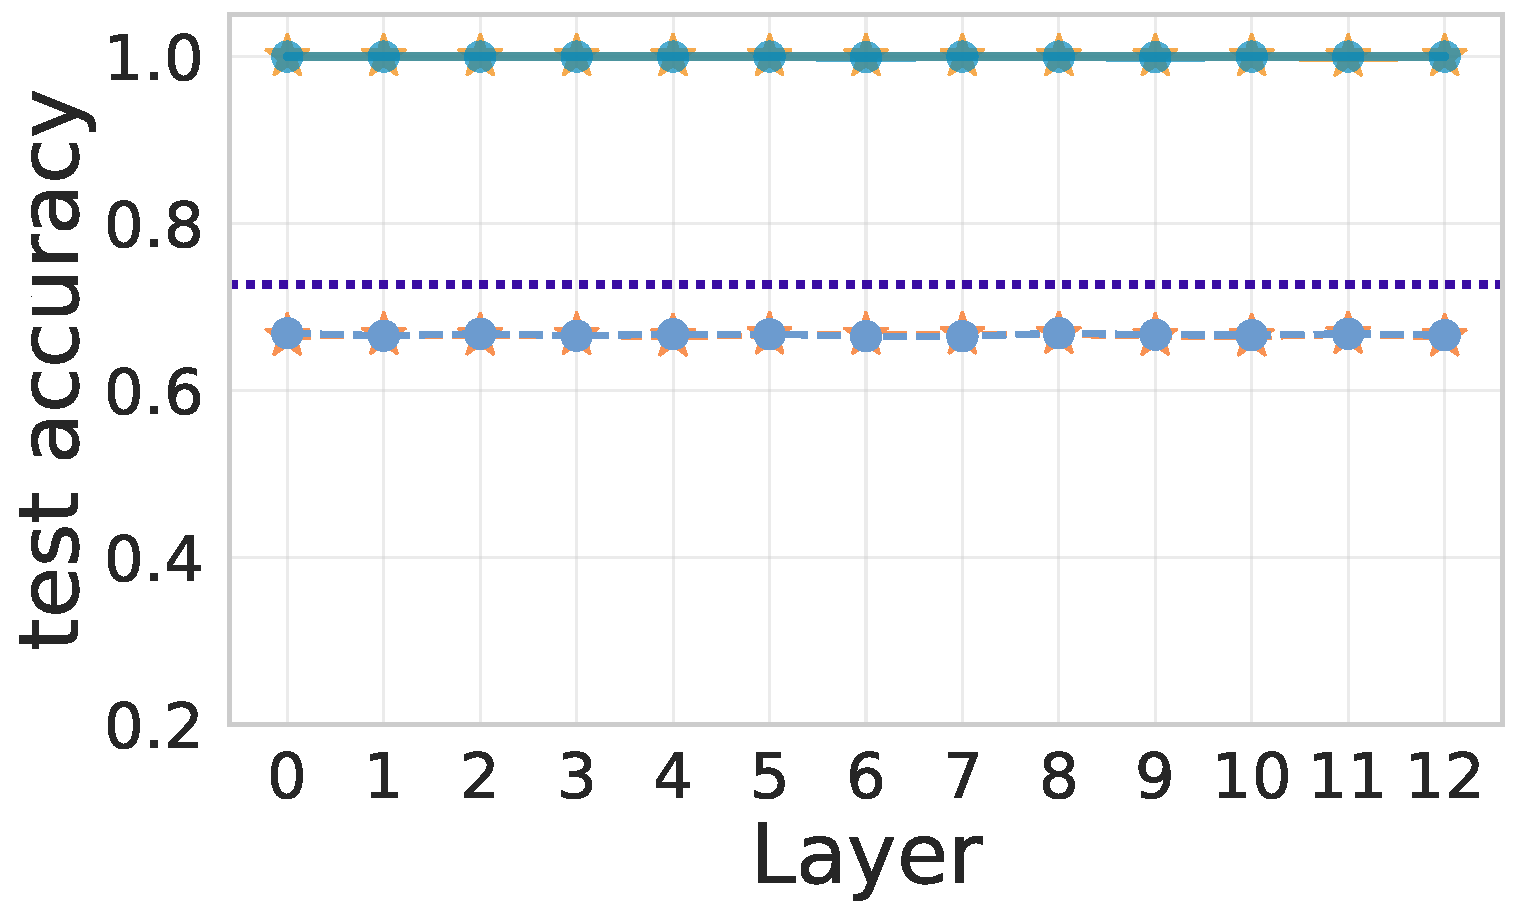
\includegraphics[width=\linewidth]{results_combined/atom_type.pdf}
    \subcaption{atom type}
    \label{fig:acc-all-atom-type}
\end{subfigure}\hfill
\begin{subfigure}[t]{0.24\linewidth}
    \centering
    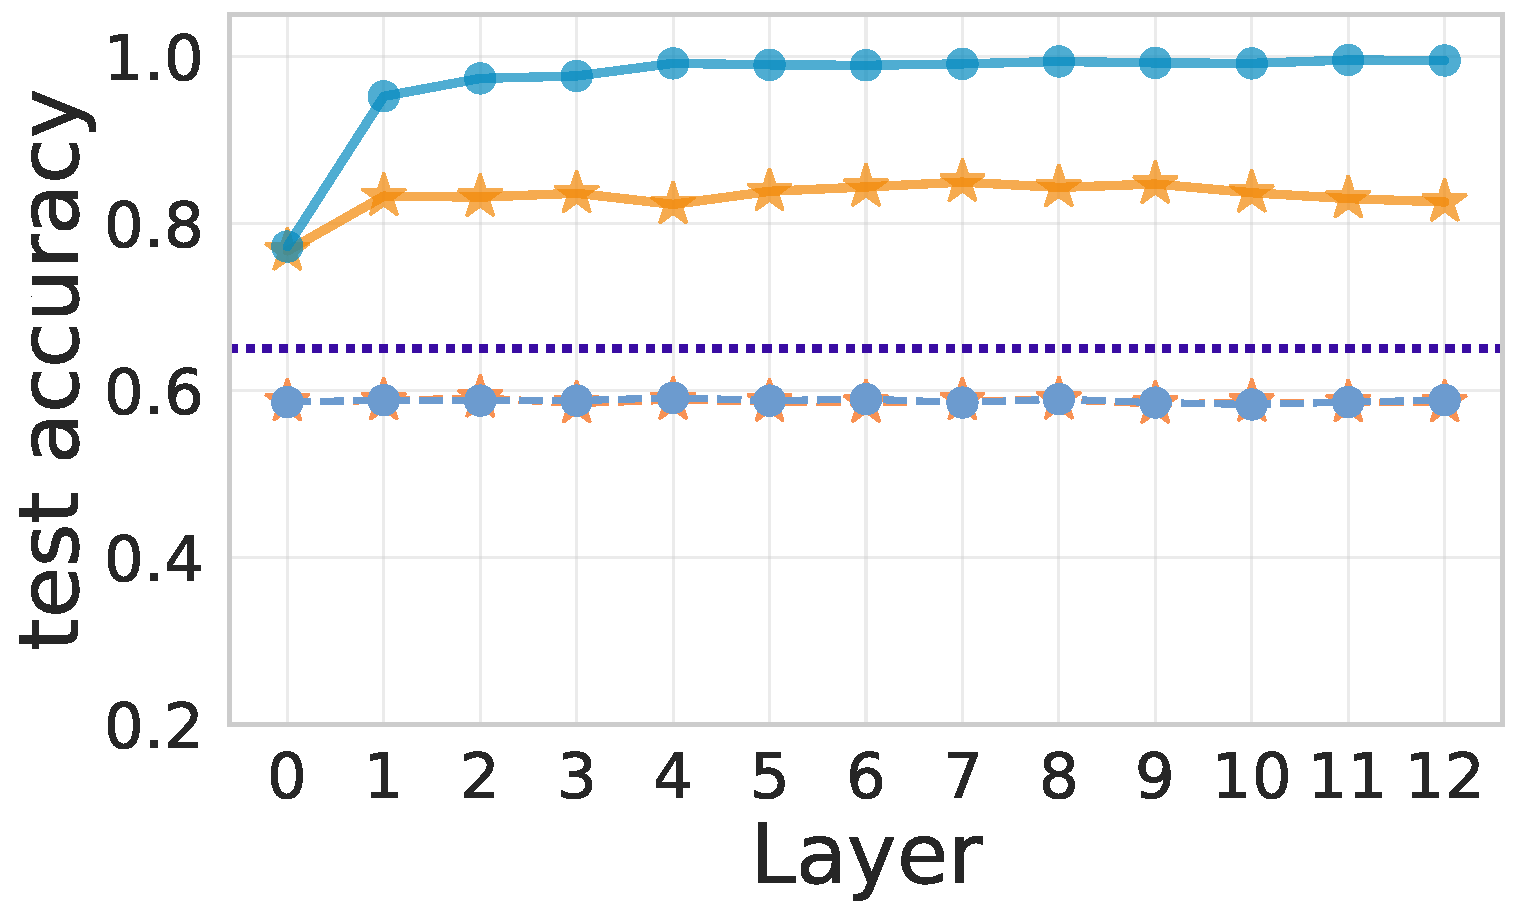
\includegraphics[width=\linewidth]{results_combined/hybridization.pdf}
    \subcaption{hybridization}
    \label{fig:acc-all-hybridization}
\end{subfigure}\hfill
\begin{subfigure}[t]{0.24\linewidth}
    \centering
    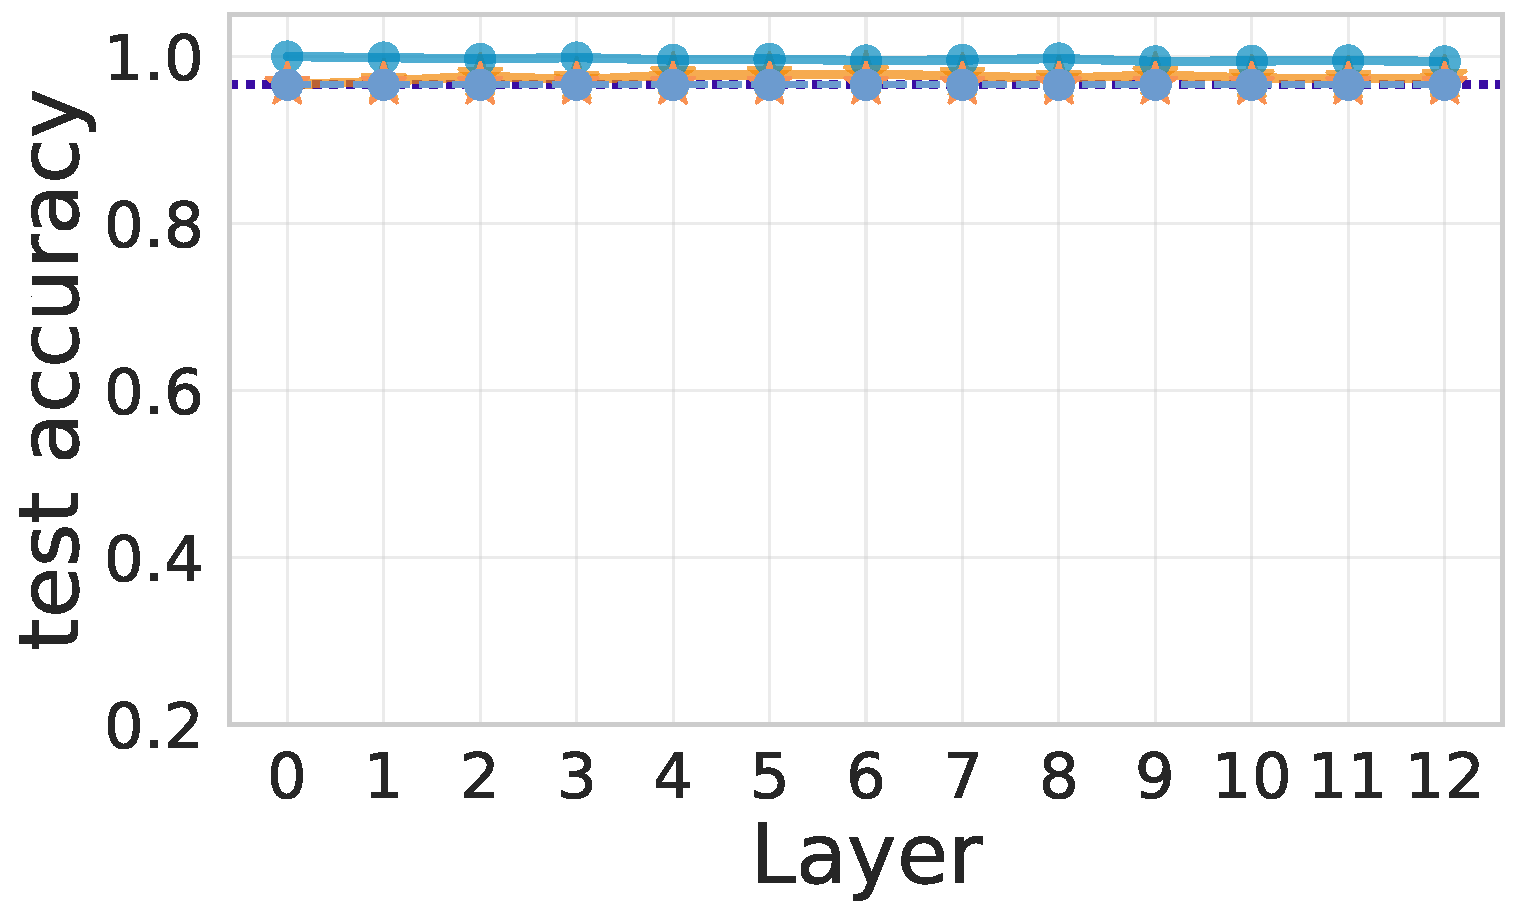
\includegraphics[width=\linewidth]{results_combined/formal_charge.pdf}
    \subcaption{formal charge}
    \label{fig:acc-all-formal-charge}
\end{subfigure}\hfill
\begin{subfigure}[t]{0.24\linewidth}
    \centering
    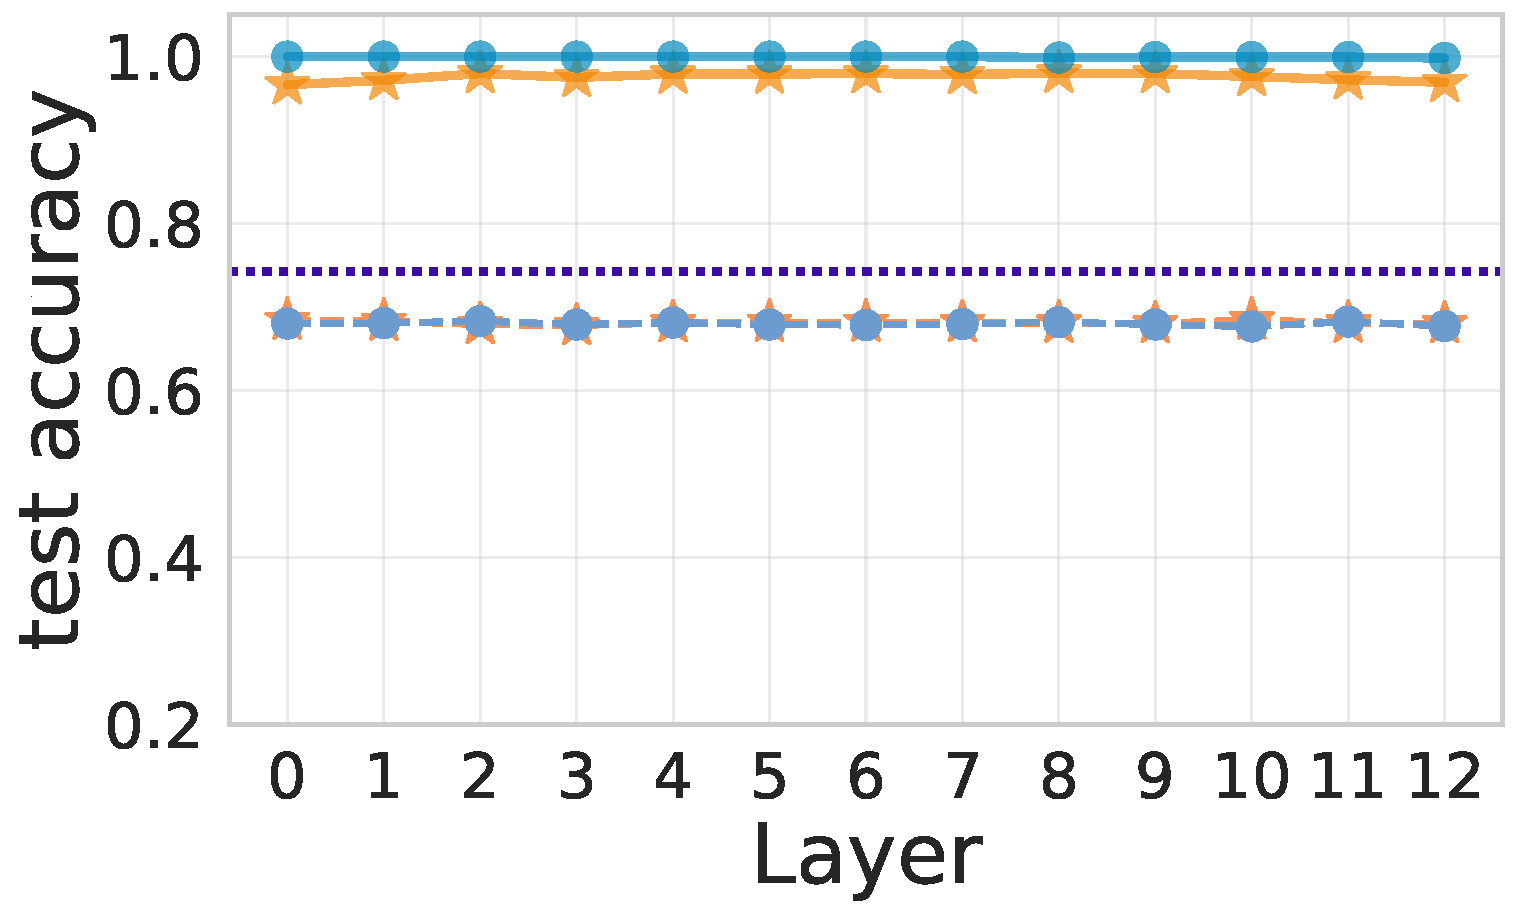
\includegraphics[width=\linewidth]{results_combined/total_valence.pdf}
    \subcaption{total valence}
    \label{fig:acc-all-total-valence}
\end{subfigure}

\vspace{0.4em}

\centerline{
\includegraphics[width=0.85\linewidth]{results_combined/legend.pdf}}

\caption{Linear-probe test accuracy per layer for the four properties not shown in the main text. Atom type (\ref{fig:acc-all-atom-type}) is surface-form and saturates at $1.0$ from layer~$0$ in both models. Formal charge (\ref{fig:acc-all-formal-charge}) is similarly close to its $0.97$ majority baseline in both models from the embedding onward. Hybridization (\ref{fig:acc-all-hybridization}) and total valence (\ref{fig:acc-all-total-valence}) are contextual and follow the same pretraining-difference shape as ring membership, degree, and chiral tag in the main text: \smi reaches near-perfect accuracy by mid-layers while \molm plateaus several points below.}
\label{fig:acc-all}
\end{figure}
\begin{figure}[t]
\centering
\begin{subfigure}[t]{0.48\linewidth}
    \centering
    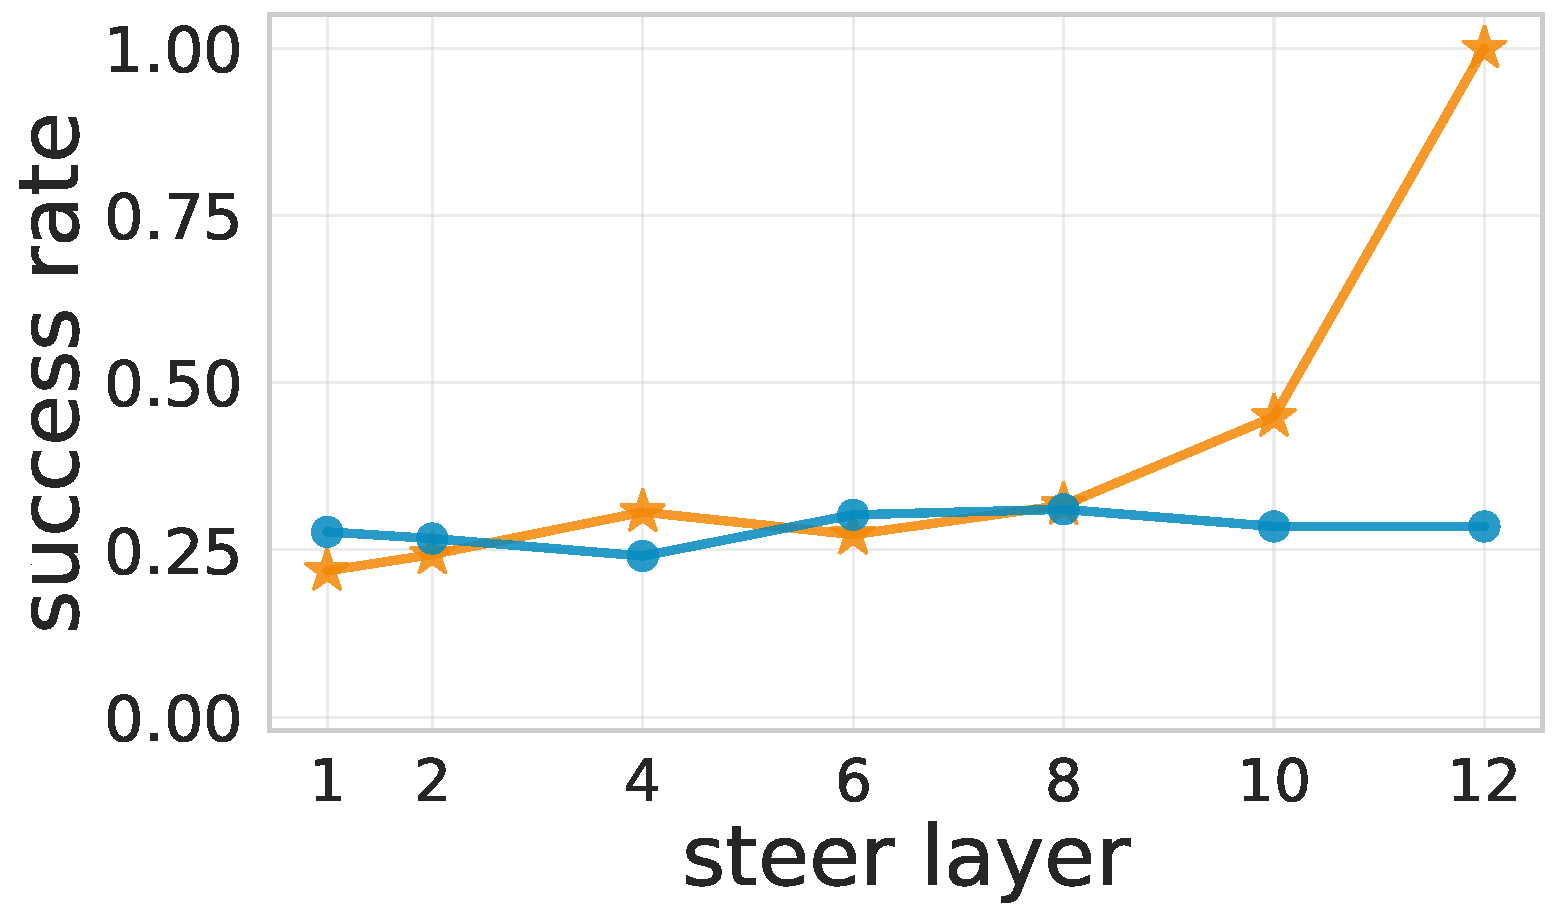
\includegraphics[width=\linewidth]{results_steer_layers/by_layer_atom_type.pdf}
    \subcaption{atom type}
    \label{fig:steer-all-atom-type}
\end{subfigure}\hfill
\begin{subfigure}[t]{0.48\linewidth}
    \centering
    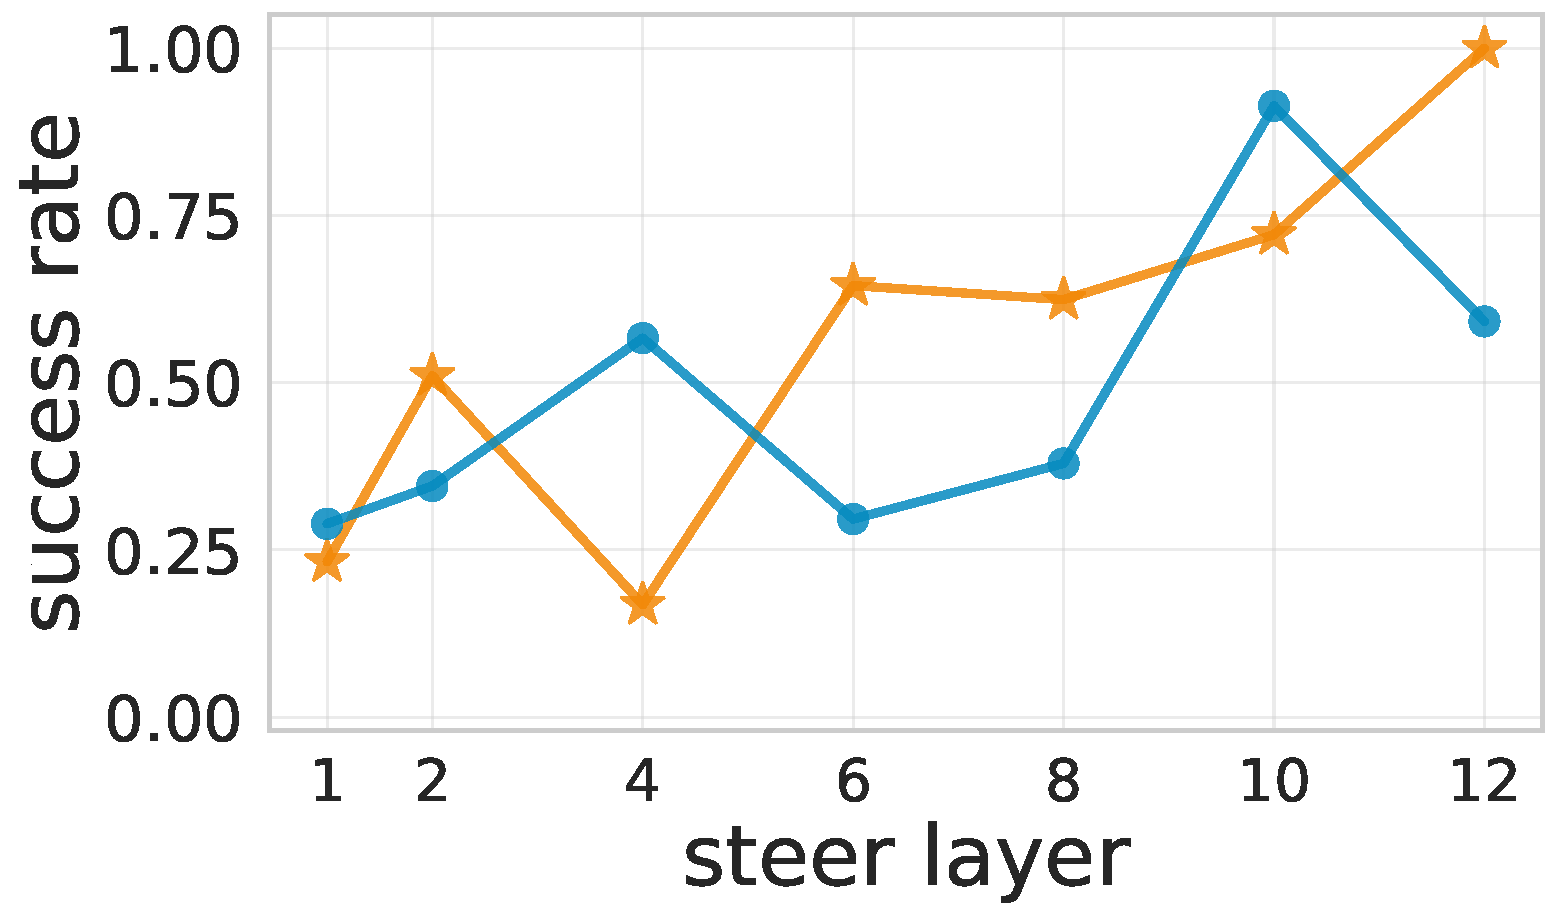
\includegraphics[width=\linewidth]{results_steer_layers/by_layer_hybridization.pdf}
    \subcaption{hybridization}
    \label{fig:steer-all-hybridization}
\end{subfigure}

\vspace{0.6em}

\begin{subfigure}[t]{0.48\linewidth}
    \centering
    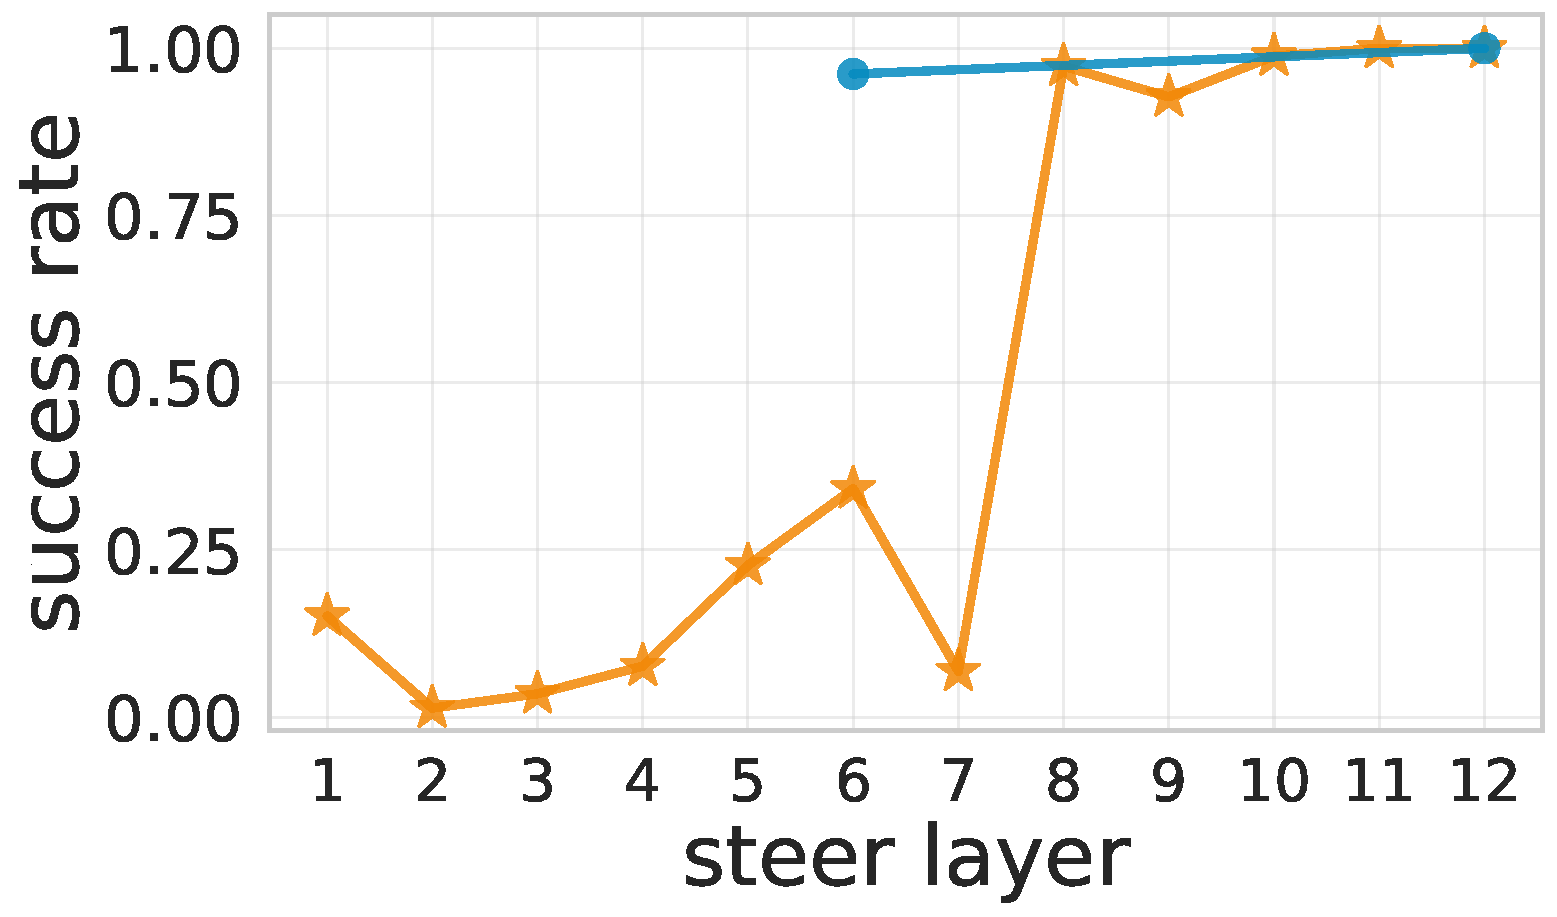
\includegraphics[width=\linewidth]{results_steer_layers/by_layer_formal_charge.pdf}
    \subcaption{formal charge}
    \label{fig:steer-all-formal-charge}
\end{subfigure}\hfill
\begin{subfigure}[t]{0.48\linewidth}
    \centering
    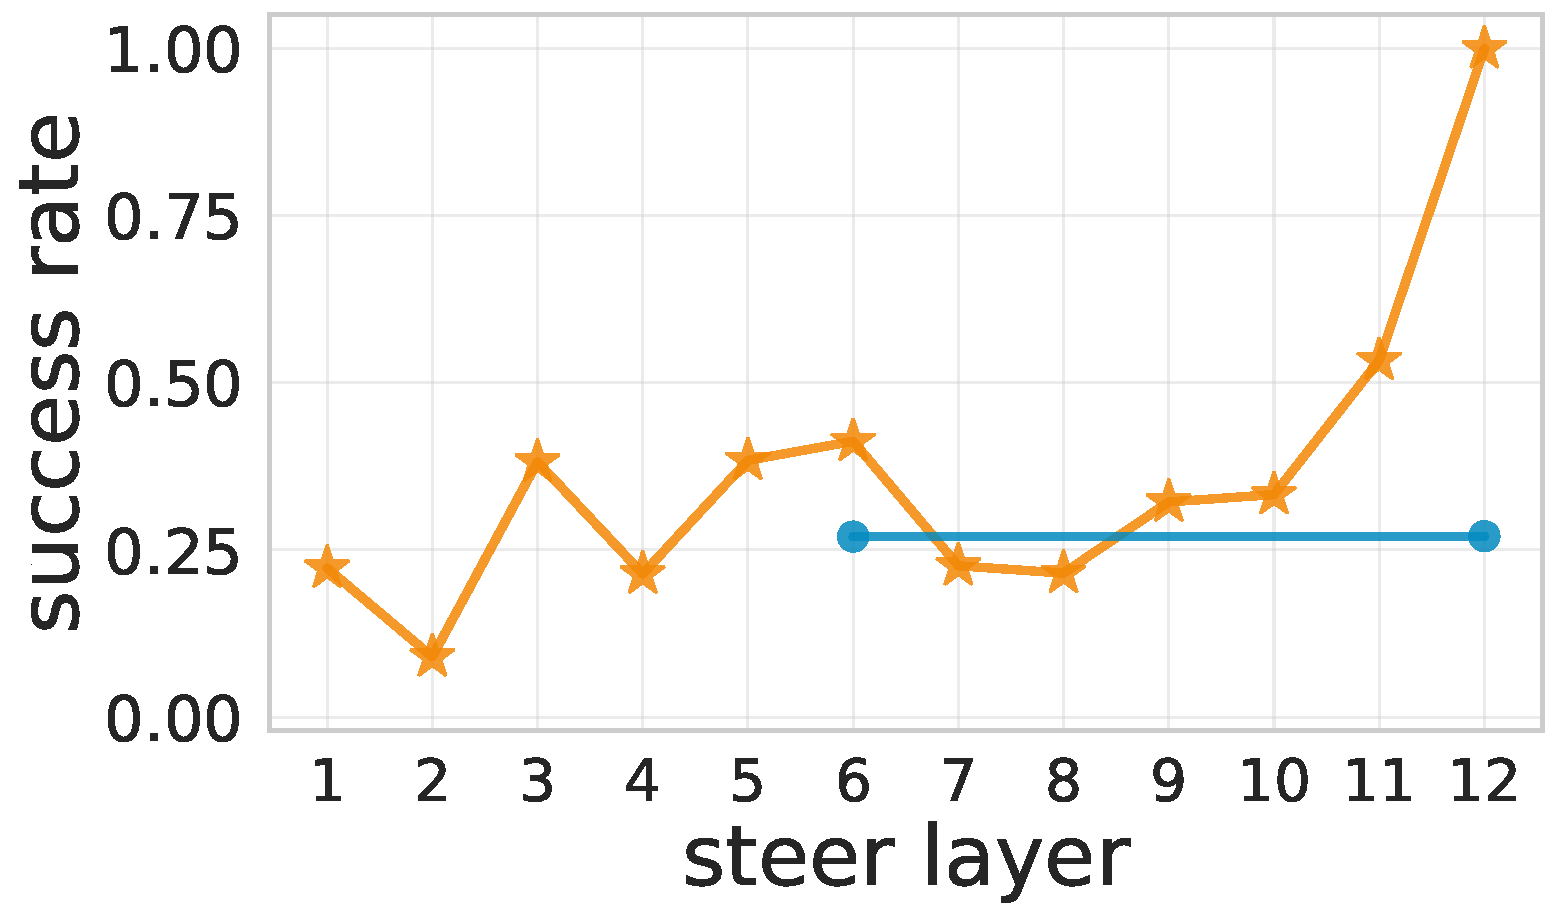
\includegraphics[width=\linewidth]{results_steer_layers/by_layer_total_valence.pdf}
    \subcaption{total valence}
    \label{fig:steer-all-total-valence}
\end{subfigure}

\vspace{0.4em}

\centerline{
\includegraphics[width=0.5\linewidth]{results_steer_layers/by_layer_legend.pdf}}

\caption{Intervention success rate as a function of the steer layer for the four properties not shown in the main text. Formal charge (\ref{fig:steer-all-formal-charge}) follows the same pretraining-difference shape seen in the main text: \smi saturates at high success by mid-layers, \molm climbs gradually until the top of the encoder. Atom type (\ref{fig:steer-all-atom-type}), hybridization (\ref{fig:steer-all-hybridization}), and total valence (\ref{fig:steer-all-total-valence}) are multi-class targets and the cycle-target success rate is partly governed by the probe-prototype layout; we therefore additionally inspect the moved-off-source rate (Appendix~\ref{app:steering}) to disentangle ``the intervention had effect'' from ``the intervention hit the cycle target''.}
\label{fig:steer-layer-all}
\end{figure}


\section{Linear Probe Training Details}
\label{app:training}

\begin{figure*}[t]
\centering
\begin{subfigure}[t]{0.24\textwidth}
    \centering
    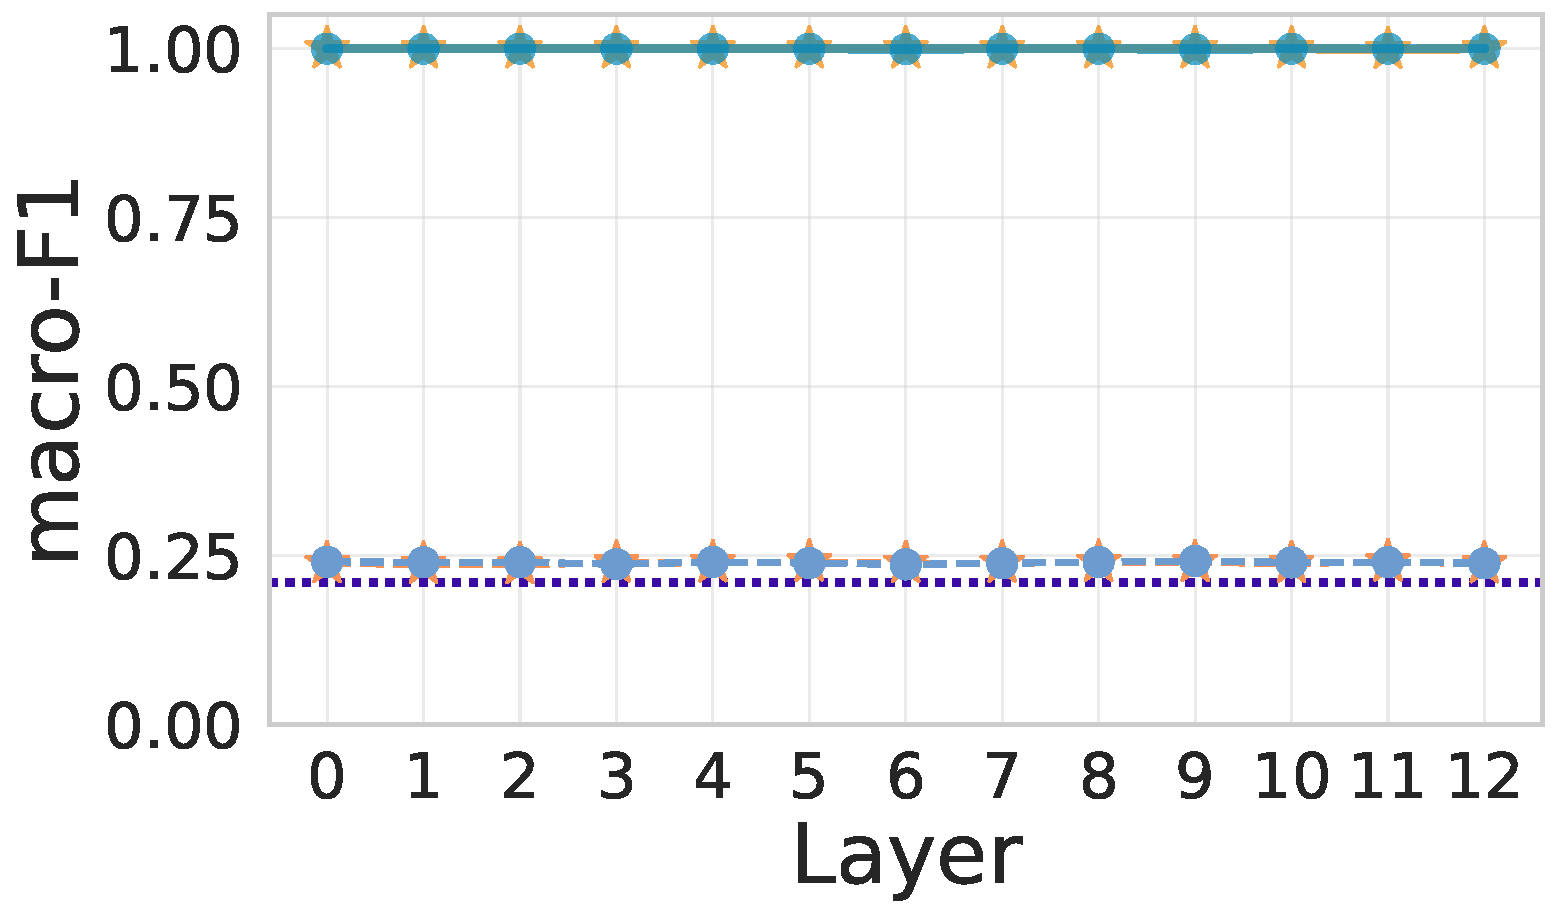
\includegraphics[width=\linewidth]{results_combined_f1/atom_type.pdf}
    \caption{atom type}
\end{subfigure}\hfill
\begin{subfigure}[t]{0.24\textwidth}
    \centering
    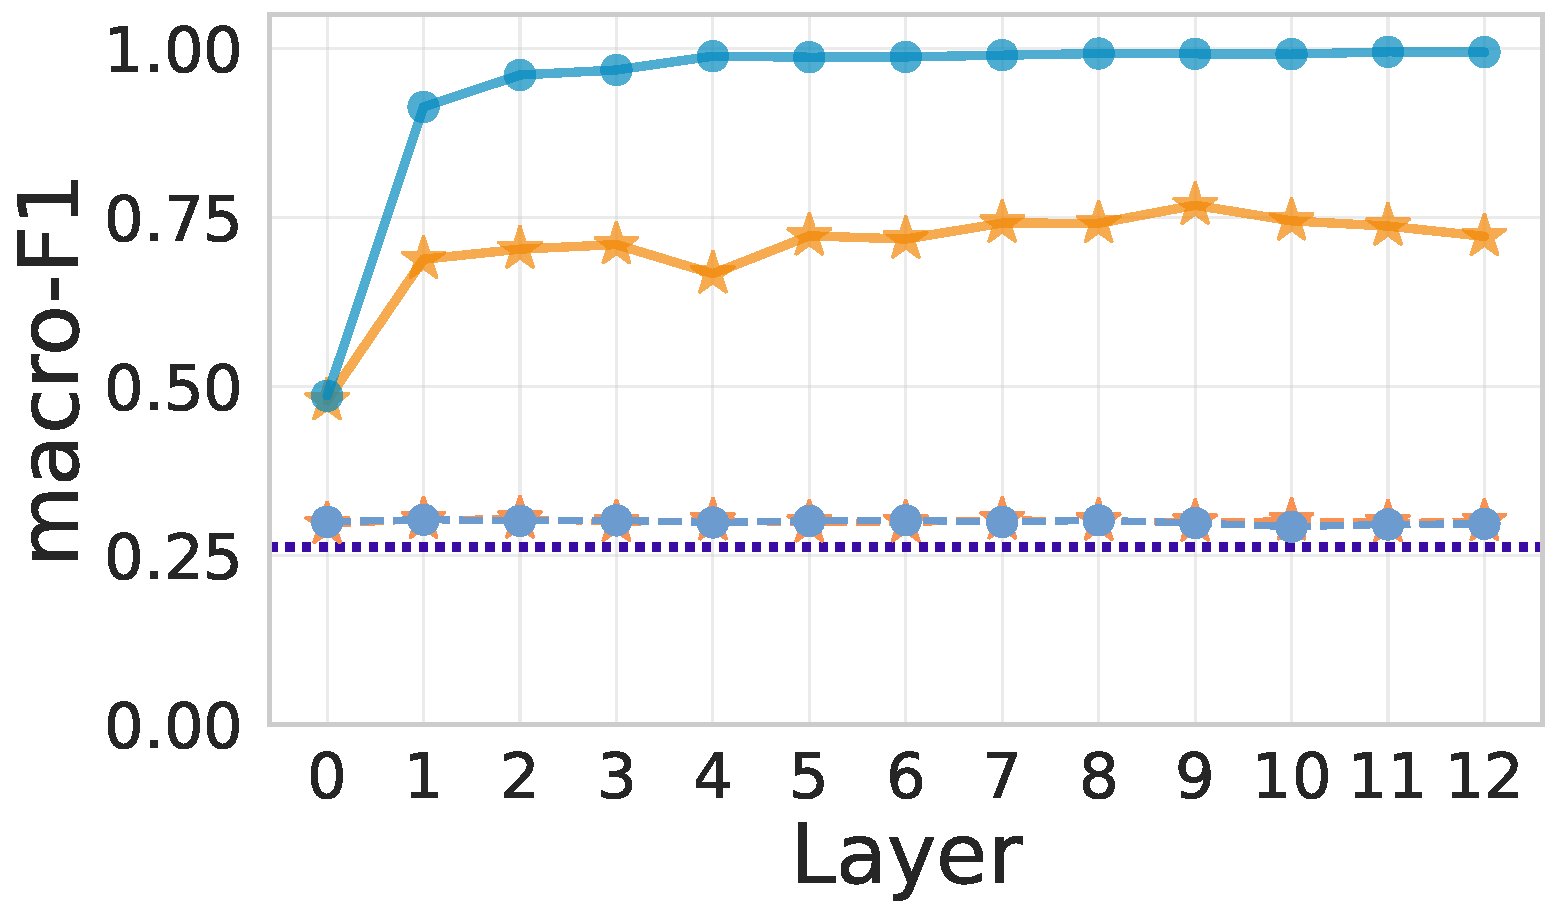
\includegraphics[width=\linewidth]{results_combined_f1/hybridization.pdf}
    \caption{hybridization}
\end{subfigure}\hfill
\begin{subfigure}[t]{0.24\textwidth}
    \centering
    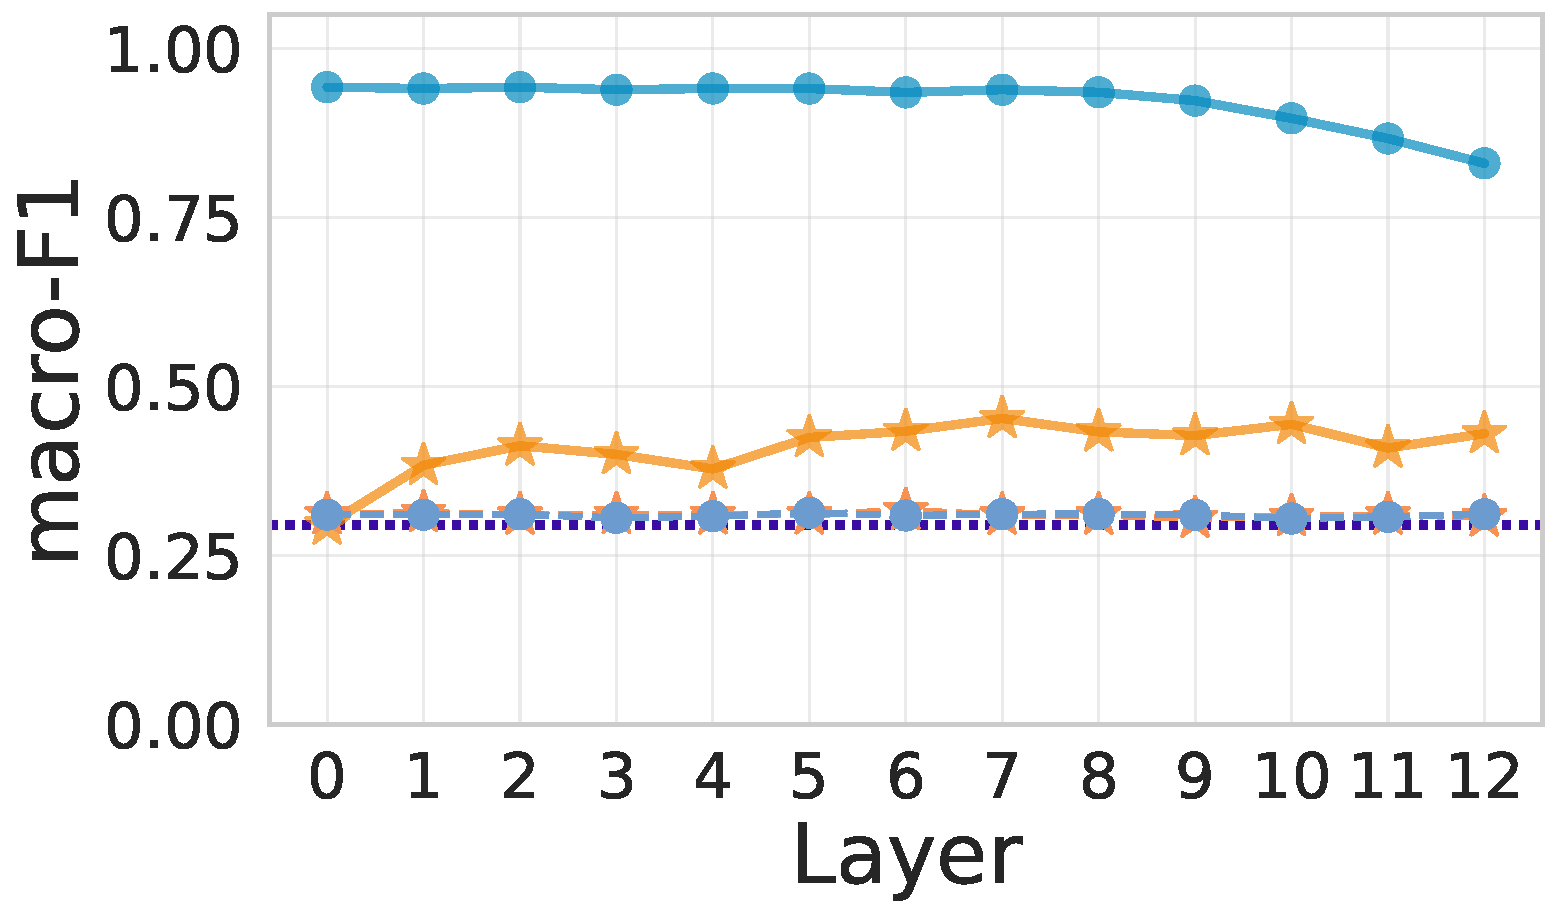
\includegraphics[width=\linewidth]{results_combined_f1/chiral_tag.pdf}
    \caption{chiral tag}
\end{subfigure}\hfill
\begin{subfigure}[t]{0.24\textwidth}
    \centering
    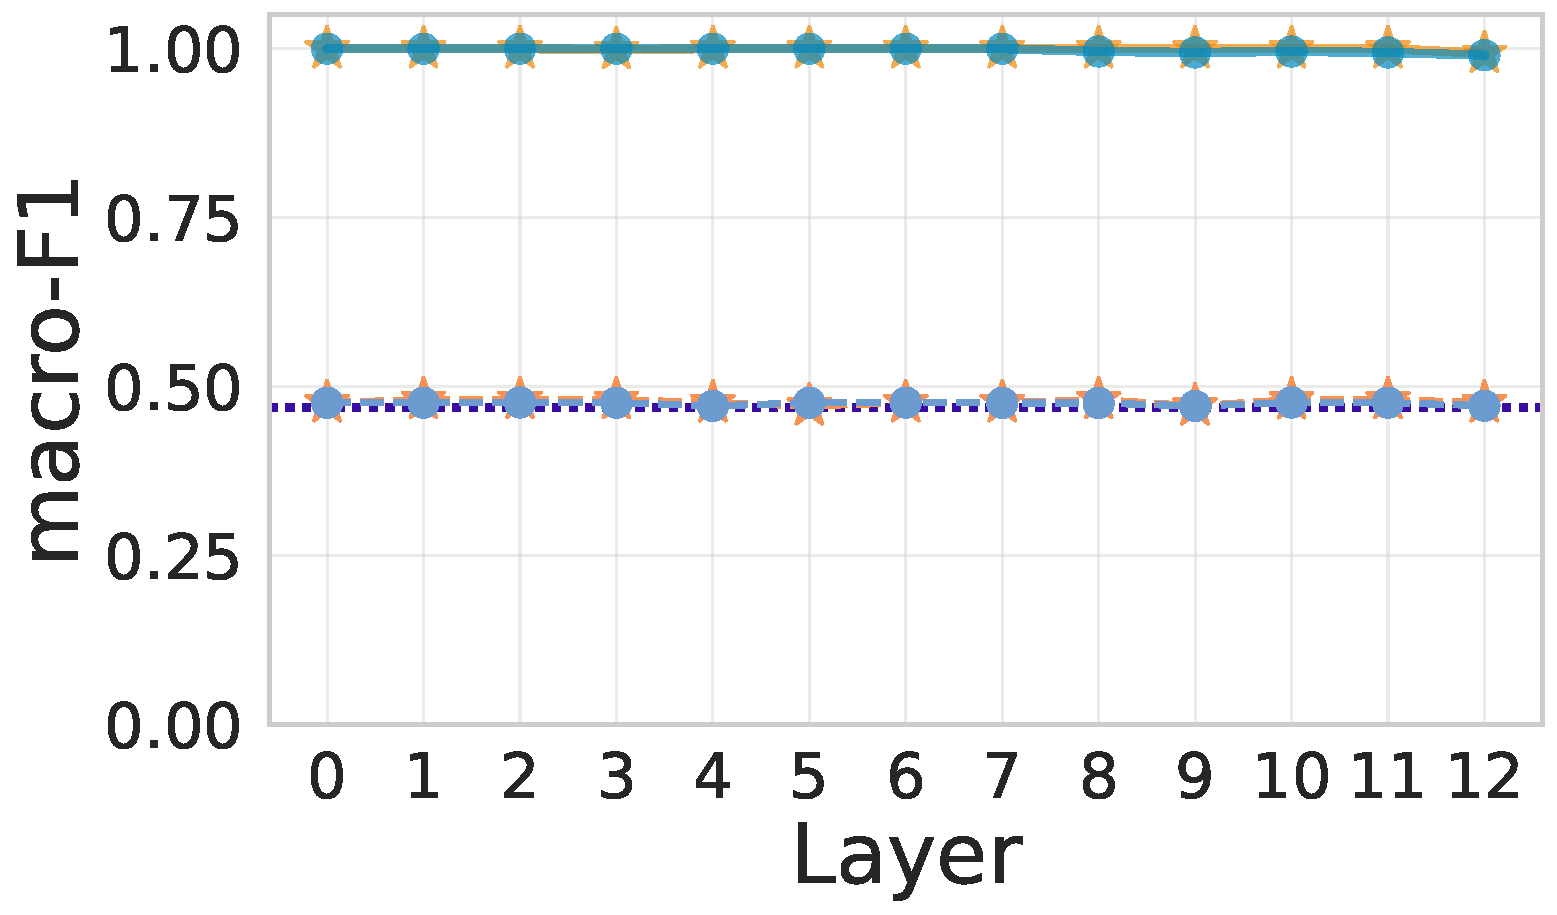
\includegraphics[width=\linewidth]{results_combined_f1/is_aromatic.pdf}
    \caption{is aromatic}
\end{subfigure}

\vspace{0.6em}

\begin{subfigure}[t]{0.24\textwidth}
    \centering
    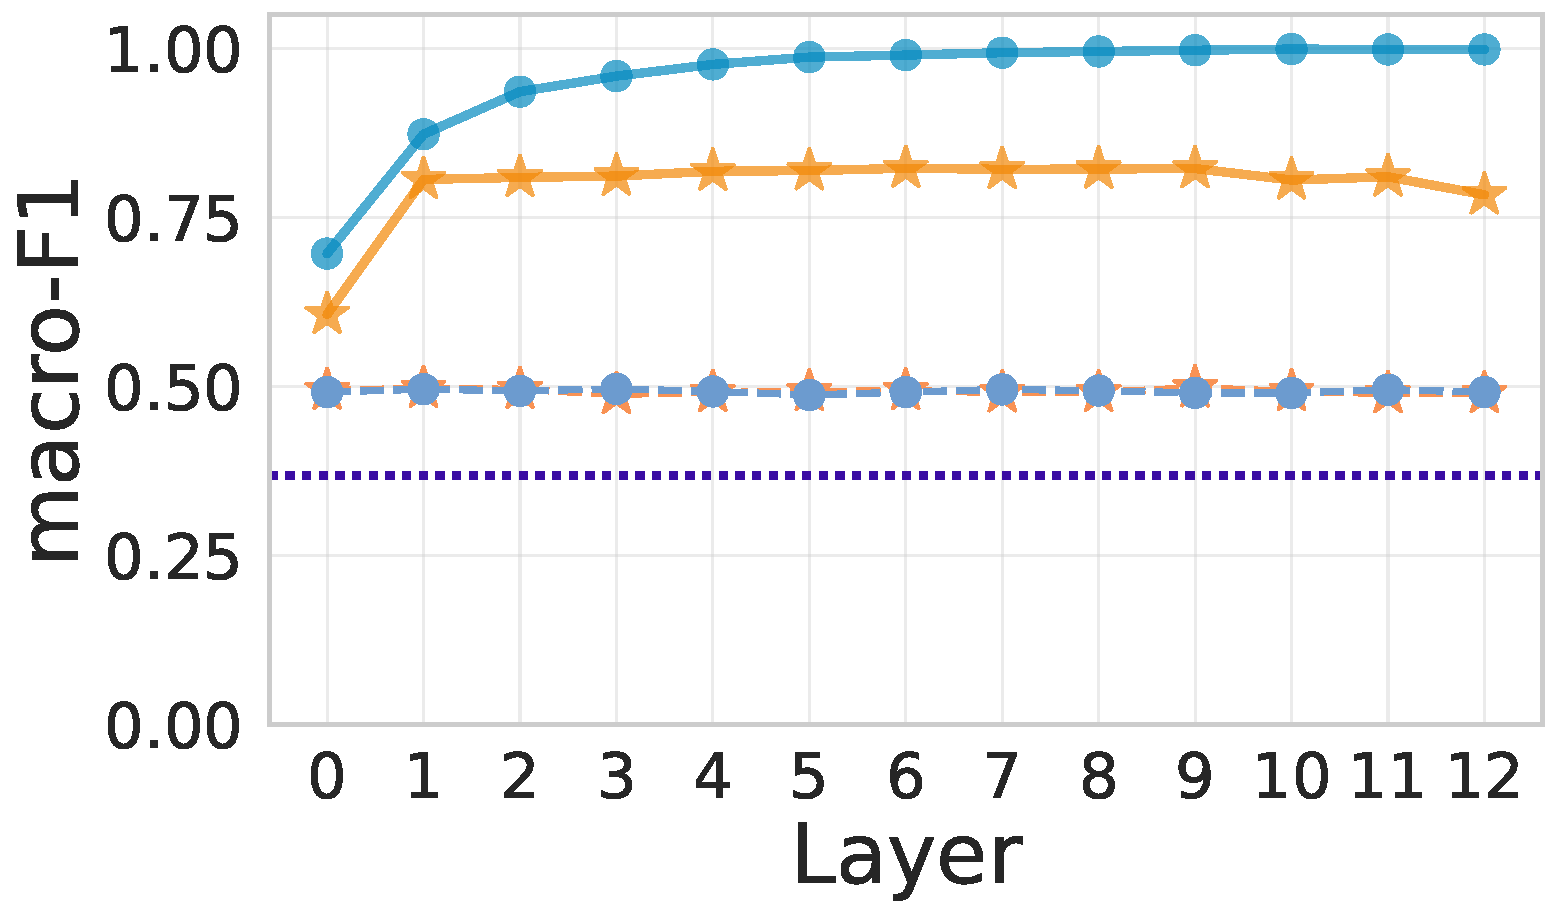
\includegraphics[width=\linewidth]{results_combined_f1/is_in_ring.pdf}
    \caption{is in ring}
\end{subfigure}\hfill
\begin{subfigure}[t]{0.24\textwidth}
    \centering
    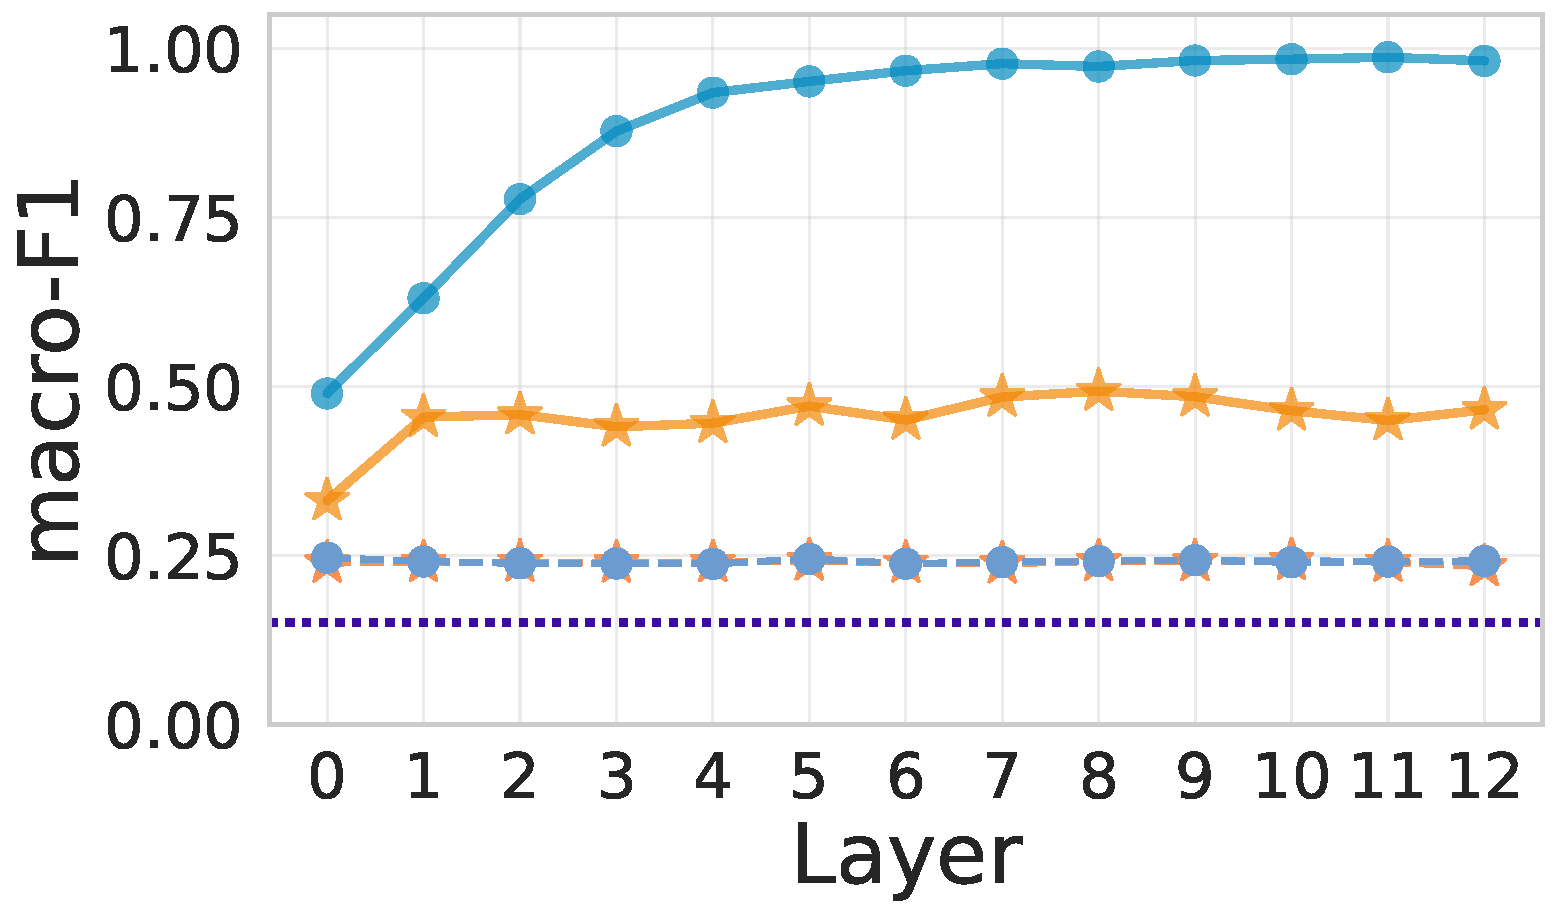
\includegraphics[width=\linewidth]{results_combined_f1/degree.pdf}
    \caption{degree}
\end{subfigure}\hfill
\begin{subfigure}[t]{0.24\textwidth}
    \centering
    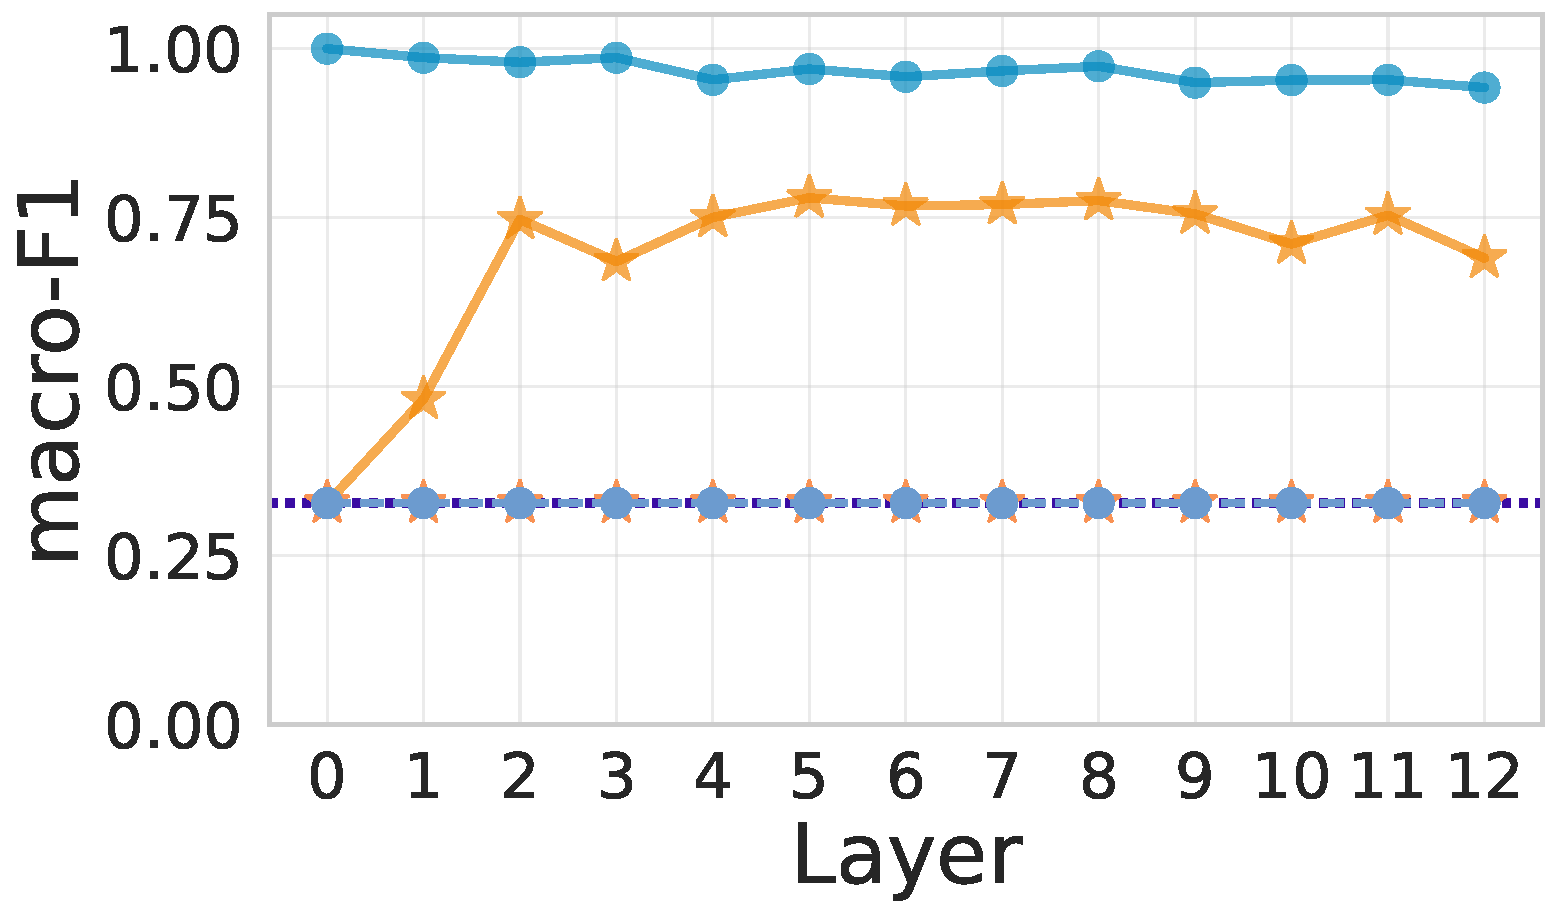
\includegraphics[width=\linewidth]{results_combined_f1/formal_charge.pdf}
    \caption{formal charge}
\end{subfigure}\hfill
\begin{subfigure}[t]{0.24\textwidth}
    \centering
    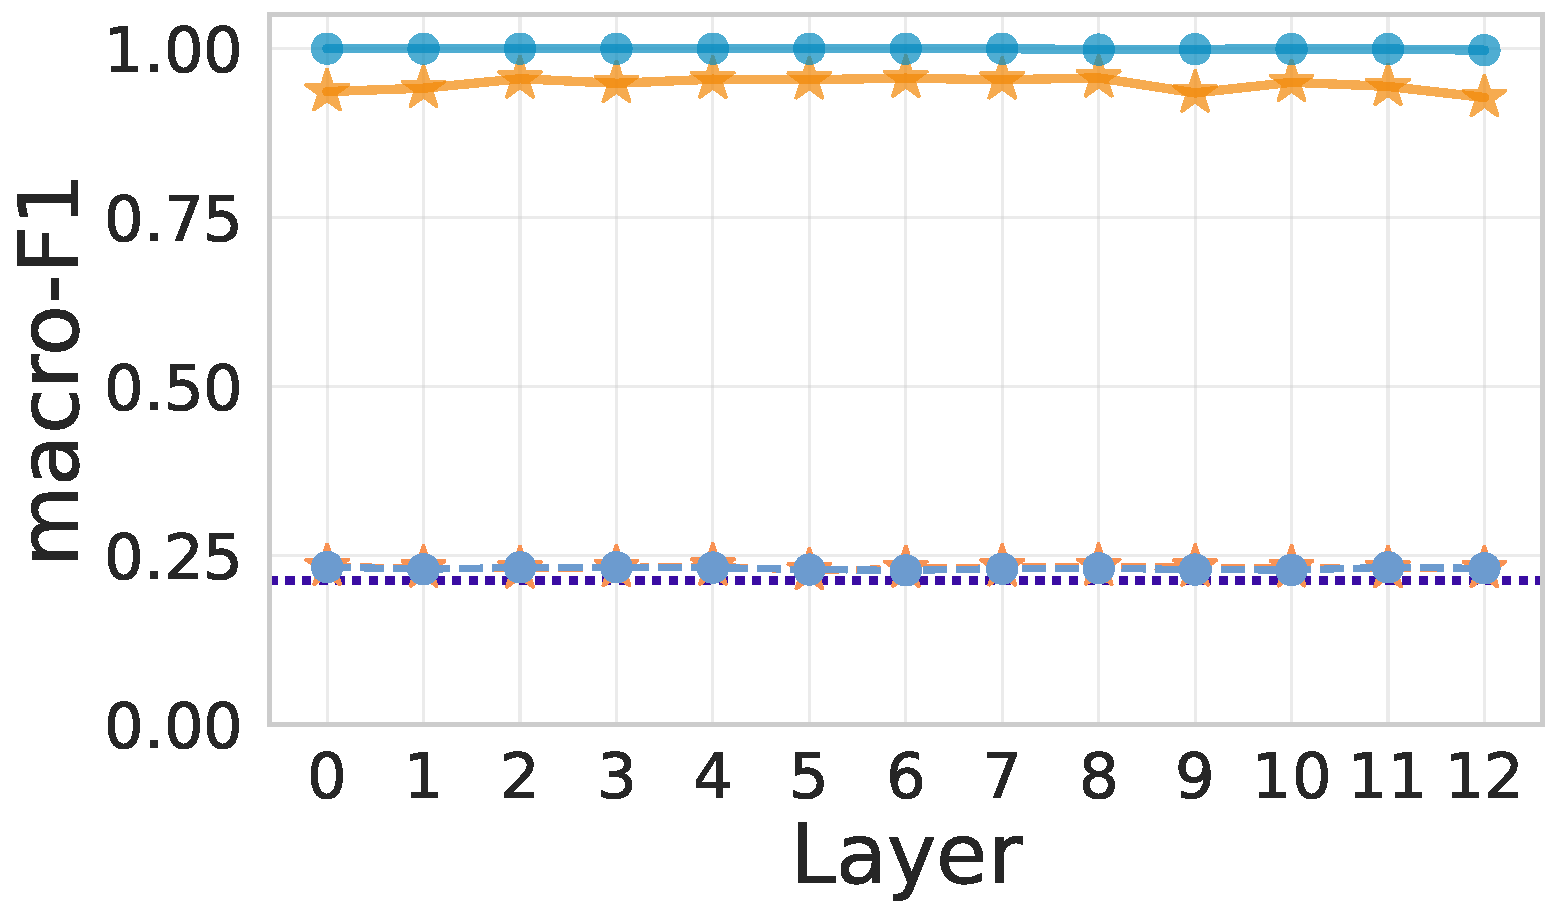
\includegraphics[width=\linewidth]{results_combined_f1/total_valence.pdf}
    \caption{total valence}
\end{subfigure}

\vspace{0.4em}

\centerline{
\includegraphics[width=0.95\textwidth]{results_combined_f1/legend.pdf}}

\caption{Per-layer linear-probe macro-F1 on the same eight tasks. Under macro-F1 \smi vs.\ \molm gap on contextual tasks is more pronounced than under accuracy, because macro-F1 penalises probes that effectively predict the majority class.}
\label{fig:f1}
\end{figure*}
\para{Optimisation.} AdamW, learning rate $10^{-3}$, weight decay $10^{-2}$, batch size $256$, $50$ epochs, gradient norm clipped at $5.0$. Probes are trained from random initialisation for every (task, layer) pair. Cross-entropy loss is unweighted; class imbalance is handled by reporting macro-F1 alongside accuracy.

\para{Data and split.} $1000$ SMILES are sampled uniformly at random from the QM9 training split (seed $42$). After RDKit parsing and atom-token alignment, approximately $980$ molecules and $\sim 8.6$k atom-token positions remain. We use a molecule-level $80/20$ split, so that no atom from a held-out molecule appears in training; this yields $\sim 6.9$k training and $\sim 1.7$k test atom-token positions. Class sets are fit on training labels only; held-out atoms whose label does not appear in training count as misclassifications and are excluded from macro-F1.

\para{Per-atom hidden-state extraction.} For each SMILES we run a forward pass with $\texttt{output\_hidden\_states=True}$, parse the molecule with RDKit, and align tokenizer-level atom tokens with their corresponding RDKit atom indices via a deterministic walk through the regex tokenization. Token-to-atom alignment is verified by checking that each atom-token's element symbol matches the corresponding RDKit atom; mismatched molecules are dropped. Each per-atom vector $\mathbf{h}^{(i)}_{\tau, l} \in \mathbb{R}^{d}$ at layer $l$ is then taken from the $i$-th atom-token row of the layer-$l$ hidden-states tensor.

\para{Standardisation.} For each (task, layer) pair, per-feature mean $\boldsymbol{\mu}_{\tau, l}$ and standard deviation $\boldsymbol{\sigma}_{\tau, l}$ are computed on the training atom-token positions only and applied as $\tilde{\mathbf{h}} = (\mathbf{h} - \boldsymbol{\mu}_{\tau, l}) / (\boldsymbol{\sigma}_{\tau, l} + 10^{-8})$ to both train and test. The $10^{-8}$ term avoids division by zero on near-constant features.

\para{Reproducibility shims.} Loading MoLFormer requires three monkey-patches against the cached HuggingFace custom code, since the public release predates \texttt{transformers}~$\geq$~5: a stub for the removed \texttt{transformers.onnx} subpackage, a stub for \texttt{find\_pruneable\_heads\_and\_indices}, and a re-injection of \texttt{PreTrainedModel.get\_head\_mask}. We also force a recomputation of the rotary embedding's non-persistent \texttt{cos\_cached}/\texttt{sin\_cached} buffers after model loading and set \texttt{deterministic\_eval=True} on every FAVOR$+$ feature map. SMI-TED's \texttt{pytorch-fast-transformers} dependency does not build under the venv we used; we reimplement its encoder in pure PyTorch ($\sim 150$ lines) and load the released checkpoint into our own modules with a strict assertion that only the post-encoder \texttt{LayerNorm} (which our probes do not read) is allowed to be unmatched.

\section{MLP Probe Control}
\label{app:mlp}

To rule out that the linear probe is bottlenecked by its lack of nonlinearity, we additionally train a 2-layer MLP probe with hidden size $128$ and ReLU activation:
\[
\mathrm{MLPProbe}(\mathbf{x}) = \mathbf{W}_2\,\mathrm{ReLU}(\mathbf{W}_1\,\mathbf{x} + \mathbf{b}_1) + \mathbf{b}_2,
\]
with $\mathbf{W}_1 \in \mathbb{R}^{128 \times 768}$ and $\mathbf{W}_2 \in \mathbb{R}^{C \times 128}$. Training hyperparameters mirror the linear probe (AdamW, $\mathrm{lr}{=}10^{-3}$, weight decay $10^{-2}$, batch size $256$, $50$ epochs, gradient clipping at $5.0$). The MLP probe and the linear probe see identical (task, layer) hidden states, splits, standardisation, and class encodings.

Across all eight tasks and both models, the MLP probe improves test accuracy over the linear probe by at most $0.03$ in absolute terms, with most improvements being $\leq 0.01$. The largest gain is on MoLFormer hybridization ($+0.03$ acc / $+0.07$ macro-F1, layer $5$); on token-determined tasks the gap is essentially zero. We conclude that the chemical properties under study are approximately linearly accessible from the residual stream and that further conclusions drawn from the linear probe are not artifacts of probe capacity.

\section{Random-Features Control}
\label{app:random}

For each (task, layer) pair we additionally train an identical linear probe on a Gaussian random-features matrix $\mathbf{X}_{\mathrm{rand}} \in \mathbb{R}^{N \times 768}$ with $\mathbf{X}_{\mathrm{rand}, ij} \sim \mathcal{N}(0, 1)$, sampled once per script run and reused for every (task, layer) random probe. The same molecule-level split, class encoding, and standardisation are applied; the probe sees the same atom labels but uninformative inputs. Test macro-F1 falls within $1$--$2$ percentage points of $1/C$ (the chance level for macro-F1 when always predicting the majority class) for every task on both models, confirming that the real-features probe accuracy reflects encoder structure rather than overfitting capacity in the linear head.

\section{Causal Steering Setup}
\label{app:steering}

\begin{table}[t]
\centering
\small
\begin{tabular}{lccc}
\toprule
Task & $C_\tau$ & \molm & \smi \\
\midrule
is aromatic   & 2 & 0.99 & 1.00 \\
is in ring    & 2 & \textbf{0.76} & \textbf{1.00} \\
chiral tag    & 3 & 0.44 & \textbf{1.00} \\
degree        & 4 & 0.64 & \textbf{0.99} \\
formal charge & 3 & 0.34 & \textbf{0.96} \\
hybridization & 3 & 0.65 & 0.30 \\
atom type     & 4 & 0.27 & 0.30 \\
total valence & 4 & 0.41 & 0.27 \\
\bottomrule
\end{tabular}
\caption{\textbf{\smi maintains probe directions through the encoder substantially better than \molm at intermediate depth.} Each cell is the success rate of a single intervention at layer~$6$ along the layer-$6$ probe direction, read by the layer-$12$ probe; bold cells indicate $\geq 0.75$ success. Binary contextual tasks (top of the table) admit a clean cross-model comparison; multi-class rows are confounded by the cycle target's dependence on the probe-prototype layout (Hypothesis~B in the text), so we additionally report depth-resolved success in Figure~\ref{fig:steer-layer}. Evaluated on $200$ held-out QM9 molecules.}
\label{tab:steering-success}
\end{table}

\para{Steering vector.} For each (task, steer layer $\ell$) we form, in the original (unstandardized) hidden-state space,
\[
\mathbf{v}^{c \to c'} = (\mathbf{W}_{c'} - \mathbf{W}_{c}) / \boldsymbol{\sigma},
\]
where $\mathbf{W}_{c}$ is the layer-$\ell$ probe's row for class $c$ and $\boldsymbol{\sigma}$ is the per-feature training standard deviation. Adding $\alpha \cdot \mathbf{v}^{c \to c'}$ to a hidden state increases the standardized logit difference $\mathrm{logit}_{c'} - \mathrm{logit}_{c}$ by $\alpha \cdot \|\mathbf{W}_{c'} - \mathbf{W}_c\|_{\boldsymbol{\sigma}^{-2}}^2$. For binary tasks, $\mathrm{tgt} = 1 - \mathrm{src}$. For multi-class tasks, we use a cycle target $\mathrm{tgt} = (\mathrm{src} + 1) \bmod C$.

\para{Forward hook and intervention.} For a steer layer $\ell$, the hook is registered on the module that produces $\mathbf{h}^{(\ell)}$ (\texttt{model.encoder.layer[$\ell$-1]} for \molm, \texttt{encoder.blocks.layers[$\ell$-1]} for \smi), modifies that layer's output by adding the per-position steering tensor at atom-token positions only, and is removed in a \texttt{try/finally} block immediately after the post-intervention forward pass. The pre- and post-intervention forward passes are run with \texttt{output\_hidden\_states=True} to capture the residual stream at every depth.

\para{Layer sweep.} The single-layer table (Table~\ref{tab:steering-success}) reports $\ell{=}6$. Figure~\ref{fig:steer-layer} (and the per-task panels in Figure~\ref{fig:steer-layer-all}) sweeps $\ell \in \{1, \ldots, 12\}$ and reports, per $(\text{task}, \text{model}, \ell)$, the intervention success rate at the best-performing $\alpha$ on the held-out molecules; this best-$\alpha$-per-layer summary is used as a single scalar diagnostic of whether the encoder routes through the layer-$\ell$ probe direction.

\para{Metrics.} \emph{Intervention success rate} (or \emph{flip-to-target rate}) is the fraction of atom-token positions whose layer-$12$ probe prediction equals the intended target $c'$ after the intervention. We additionally report \emph{moved-off-source rate} (the fraction whose post-intervention layer-$12$ prediction differs from the source class $c$) so that, for multi-class tasks, ``steering had effect'' can be disentangled from ``steering hit the intended target''---a distinction that matters when the cycle target $\mathbf{W}_{c'}-\mathbf{W}_{c}$ does not point at the cycle-target centroid in the probe's prototype layout.

\para{Sample size and hyperparameters.} Each task is evaluated on $200$ molecules ($\sim 1.7$k atoms) drawn from the QM9 partition not used for probe training. The $\alpha$ grid is $\{0, 1, 3, 10, 30, 100, 300\}$; the smallest non-zero $\alpha$ that maximizes success rate is reported per layer.
